\chapter{State of the Art}

This chapter reviews the technical foundations underlying this thesis: regression modeling approaches for tabular data, feature selection methodologies, and the SHAP framework with particular attention to TreeExplainer. The review establishes both the theoretical background and practical considerations that inform the experimental design.

\section{Regression Modeling for Tabular Data}

Tabular data, structured records with rows representing observations and columns representing features, remains the dominant format in business and scientific applications. Unlike images or text, tabular datasets present heterogeneous feature types, varying scales, and often complex correlation structures that require careful modeling choices.

\subsection{Linear Models}

Regularized linear regression, particularly Ridge regression~\cite{hoerl1970ridge}, provides a baseline approach with well-understood properties. Ridge regression minimizes the sum of squared residuals plus an L2 penalty on coefficient magnitudes:

\begin{equation}
\hat{\beta} = \arg\min_{\beta} \left( \|y - X\beta\|^2 + \lambda\|\beta\|^2 \right)
\end{equation}

This formulation shrinks coefficients toward zero without eliminating them entirely, providing some implicit feature weighting. Linear models are computationally efficient and interpretable, but may underperform when relationships between features and target are nonlinear.

\subsection{Ensemble Tree Methods}

Tree-based ensembles have become the dominant approach for tabular regression~\cite{breiman2001random}. Two architectures are particularly relevant:

\textbf{Bagging ensembles}, exemplified by ExtraTrees (Extremely Randomized Trees)~\cite{geurts2006extremely}, construct multiple decision trees on bootstrap samples with additional randomization in split selection. By averaging predictions across trees, these methods reduce variance while maintaining the ability to capture nonlinear relationships and feature interactions.

\textbf{Gradient boosting}, exemplified by XGBoost~\cite{chen2016xgboost}, builds trees sequentially where each tree corrects the residual errors of its predecessors. This additive training approach often achieves state-of-the-art performance on structured data, though it introduces more hyperparameters and potential for overfitting compared to bagging methods.

Both ensemble types provide native feature importance measures: for bagging ensembles, importance typically reflects how often a feature is used in splits weighted by the improvement achieved; for gradient boosting, importance can be measured by gain (total reduction in loss from splits using that feature), weight (split frequency), or cover (number of samples affected).

\section{Feature Selection Strategies}

Feature selection methods are conventionally categorized into three families based on their relationship with the learning algorithm~\cite{guyon2003introduction}.

\subsection{Filter Methods}

Filter methods evaluate features independently of any specific model, typically using statistical measures of relevance. Mutual Information (MI) is a widely used filter criterion that captures arbitrary dependencies between a feature $X$ and target $Y$:

\begin{equation}
MI(X; Y) = \sum_{x,y} p(x,y) \log \frac{p(x,y)}{p(x)p(y)}
\end{equation}

For continuous variables, MI is estimated through discretization or kernel density methods. Filter methods are computationally cheap and model-agnostic, but ignore feature interactions and may select redundant variables.

\subsection{Wrapper Methods}

Wrapper methods evaluate feature subsets by training the target model and measuring performance. Recursive Feature Elimination (RFE) is a prominent example: starting with all features, RFE iteratively removes the least important feature(s) according to the model's own importance scores, continuing until a desired subset size is reached. While wrapper methods account for model-specific behavior, they are computationally expensive and may overfit to the evaluation metric.

\subsection{Embedded Methods}

Embedded methods perform selection as part of model training. L1-regularized regression (Lasso)~\cite{tibshirani1996lasso} is the canonical example, where the penalty term drives some coefficients exactly to zero. Tree-based models also embed implicit selection by only splitting on informative features. This thesis treats tree-based native importance as an embedded approach, though it can also serve as input to explicit subset selection.

\section{SHAP: Theory and Computation}

SHAP (SHapley Additive exPlanations)~\cite{lundberg2017unified} provides a unified framework for feature attribution that satisfies desirable theoretical properties from cooperative game theory. Understanding SHAP requires examining both its theoretical foundations and practical computational approaches.

\subsection{Shapley Values in Feature Attribution}

The core idea borrows from cooperative game theory, where Shapley values~\cite{shapley1953value} fairly distribute a total payoff among players according to their marginal contributions. In the feature attribution context, features are ``players'' and the ``payoff'' is the model prediction minus a baseline (typically the expected prediction).

For a model $f$, the Shapley value $\phi_j$ for feature $j$ is defined as:

\begin{equation}
\phi_j = \sum_{S \subseteq N \setminus \{j\}} \frac{|S|!(|N|-|S|-1)!}{|N|!} \left[ f(S \cup \{j\}) - f(S) \right]
\end{equation}

where $N$ is the set of all features, $S$ is a subset excluding feature $j$, and $f(S)$ represents the model prediction when only features in $S$ are ``present'' (with absent features marginalized out). This formula averages the marginal contribution of feature $j$ over all possible orderings in which features could be added.

Shapley values uniquely satisfy four axioms~\cite{fryer2021shapley}:
\begin{itemize}
    \item \textbf{Efficiency}: attributions sum to the difference between the prediction and baseline.
    \item \textbf{Symmetry}: features with identical contributions receive identical attributions.
    \item \textbf{Dummy}: features that never change predictions receive zero attribution.
    \item \textbf{Linearity}: attributions combine linearly across additive models.
\end{itemize}

For feature selection, global importance is typically computed by averaging absolute SHAP values across all observations: $I_j = \frac{1}{n}\sum_{i=1}^{n}|\phi_j^{(i)}|$.

\subsection{TreeExplainer: Efficient SHAP for Tree Ensembles}

The na\"ive computation of Shapley values requires evaluating exponentially many feature subsets, which is intractable for high-dimensional data. TreeExplainer~\cite{lundberg2020local} exploits the structure of decision trees to compute exact SHAP values in polynomial time.

The key insight is that a decision tree already partitions the feature space into regions, and the path from root to leaf for any observation defines which features were used. TreeExplainer recursively propagates SHAP values through the tree structure, correctly handling the exponential number of coalitions by clever bookkeeping of how predictions change as features are revealed or hidden.

For an ensemble of $T$ trees, each with $L$ leaves and average depth $D$, TreeExplainer computes exact SHAP values in $O(TLD^2)$ time per observation. Here, $T$ is the number of trees in the ensemble, $L$ is the number of leaves per tree, and $D$ is the tree depth. This is dramatically faster than model-agnostic approaches but still represents non-trivial overhead compared to simply extracting native importance scores.

\subsection{Practical Considerations}

Several factors affect SHAP computation in practice:

\textbf{Sample size}: computing SHAP for all training observations may be expensive; practitioners often use a representative sample.

\textbf{Background data}: SHAP values depend on a reference distribution used to marginalize absent features. TreeExplainer typically uses the training data itself as background.

\textbf{Stability}: because tree ensembles are stochastic (due to random splits or bootstrap sampling), SHAP rankings may vary between model fits, potentially affecting selection consistency.

\section{Datasets for Evaluation}

Before running long experiments, a pre-study pipeline was executed to download, preprocess, and characterize each dataset. This section summarizes the four datasets selected for the broad benchmark, chosen to span different scales and correlation structures.

\begin{table}[h]
\centering
\caption{Dataset characteristics after preprocessing.}
\label{tab:datasets}
\begin{tabular}{lrrrrl}
\toprule
\textbf{Dataset} & \textbf{Rows} & \textbf{Num.} & \textbf{Cat.} & \textbf{Target} & \textbf{Domain} \\
\midrule
Allstate Claims~\cite{gaurallstate} & 188,318 & 14 & 116 & loss & Insurance \\
Bike Sharing~\cite{fanaee2014event} & 17,379 & 12 & 0 & cnt & Rentals \\
Communities \& Crime~\cite{redmond2002data} & 1,993 & 100 & 0 & ViolentCrimesPerPop & Crime \\
Superconductor~\cite{hamidieh2018superconductor} & 21,263 & 81 & 0 & critical\_temp & Materials \\
\bottomrule
\end{tabular}
\end{table}

This collection provides diversity along several axes:

\textbf{Scale}: from under 2,000 observations (Communities and Crime) to nearly 200,000 (Allstate), testing whether method behavior differs with sample size.

\textbf{Dimensionality}: from 12 features (Bike Sharing) to 130 features (Allstate), covering both low and high-dimensional regimes.

\textbf{Correlation structure}: the pre-study correlation heatmaps reveal that some datasets exhibit strong feature clusters (Communities and Crime) while others show more dispersed correlation patterns.

\begin{figure}[p]
    \centering
    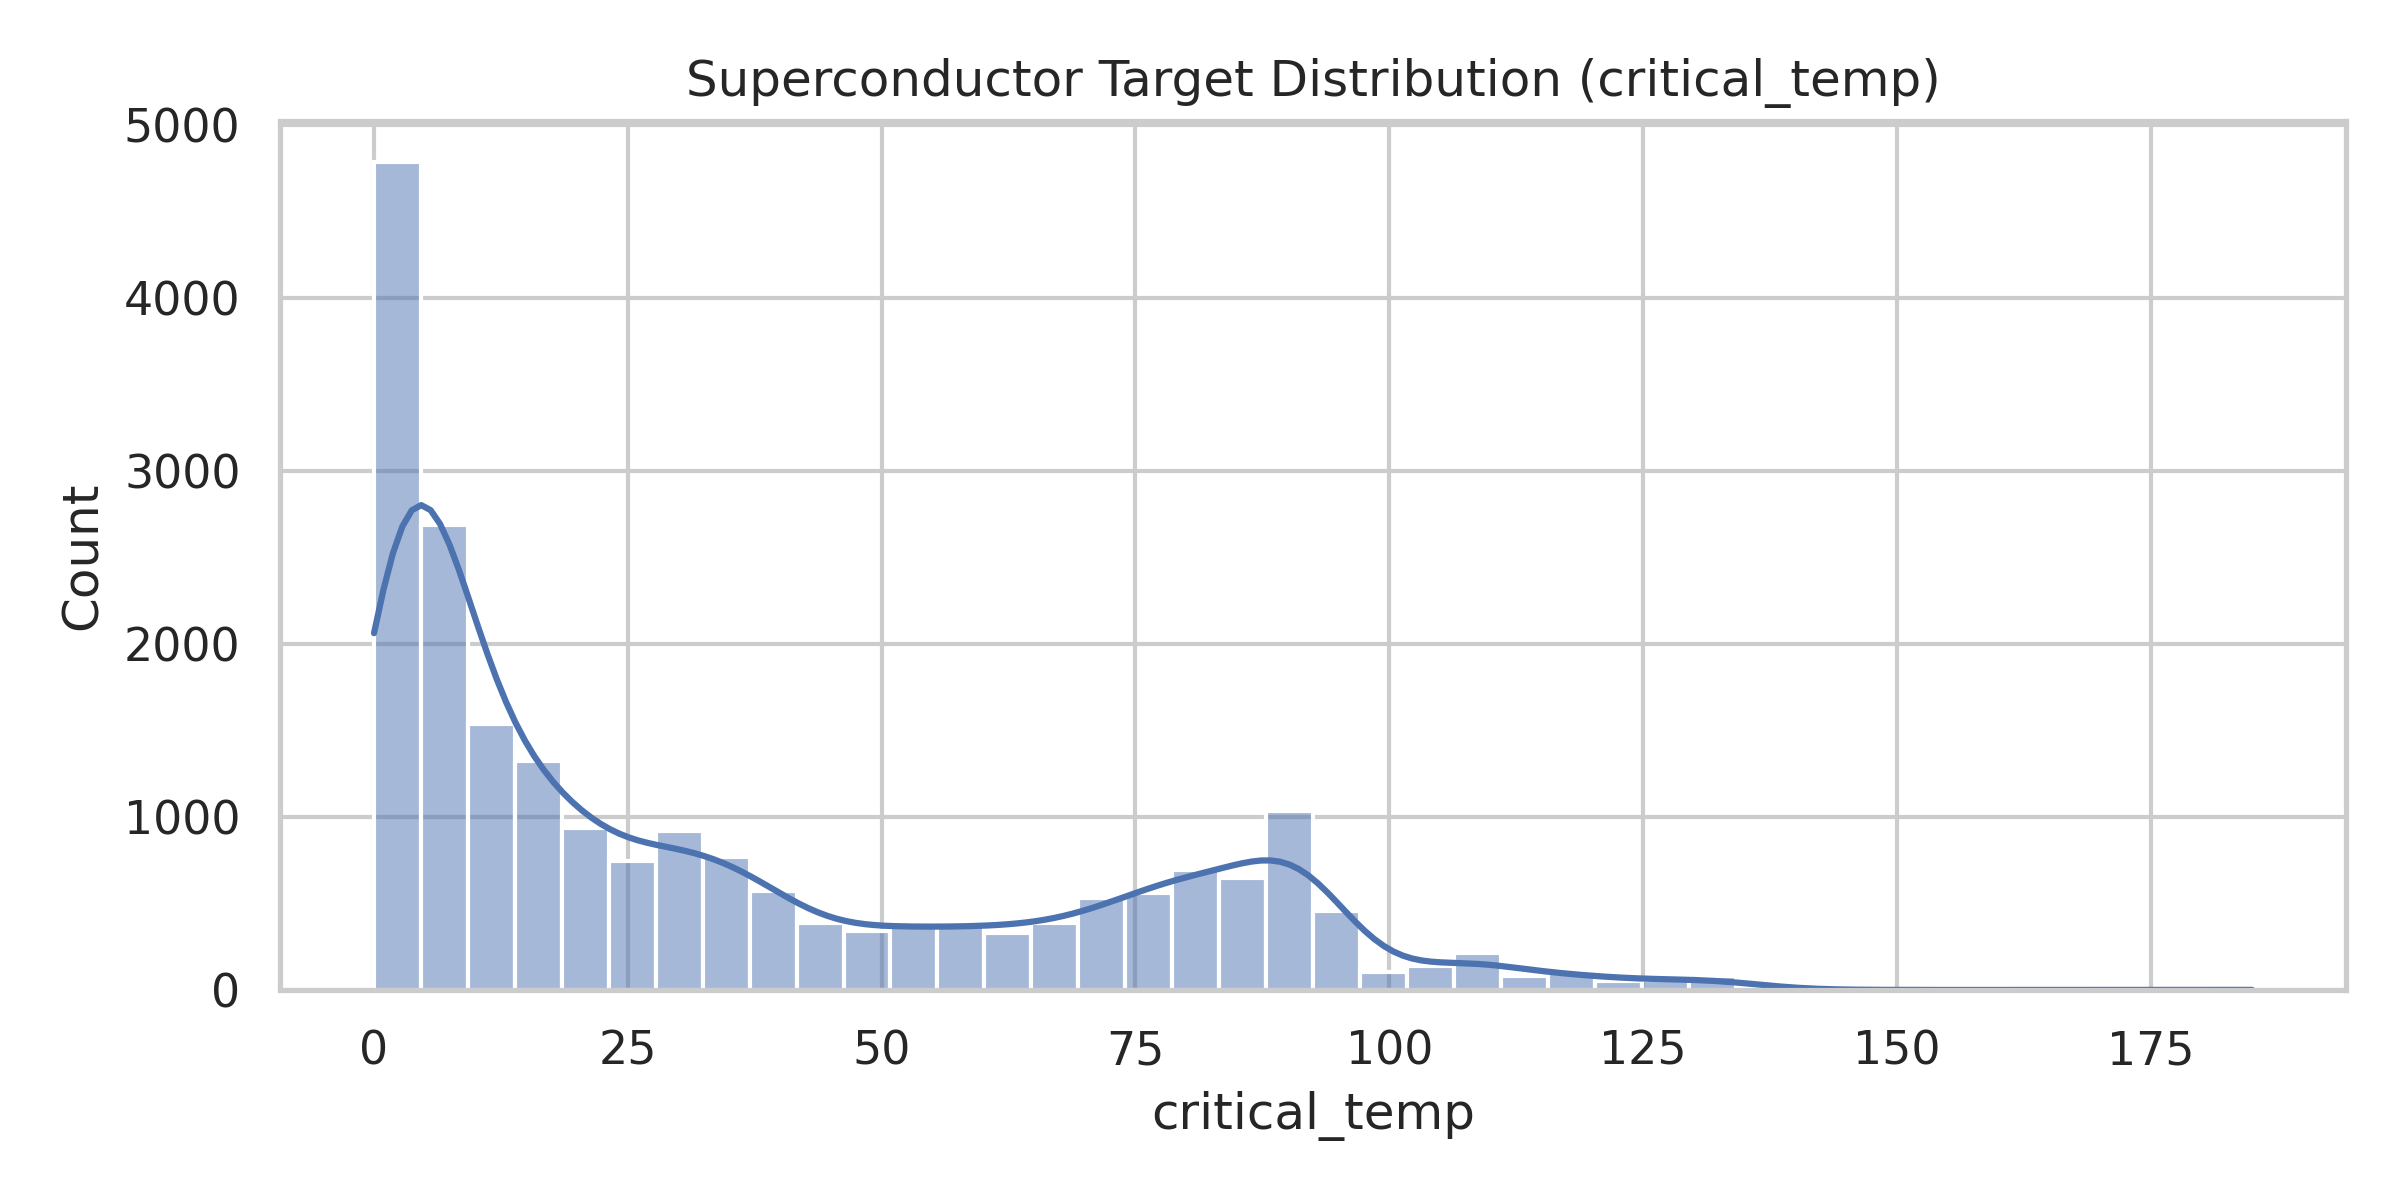
\includegraphics[width=0.65\textwidth]{../pre_study/figures/superconductor_target_distribution.png}\\[0.3em]
    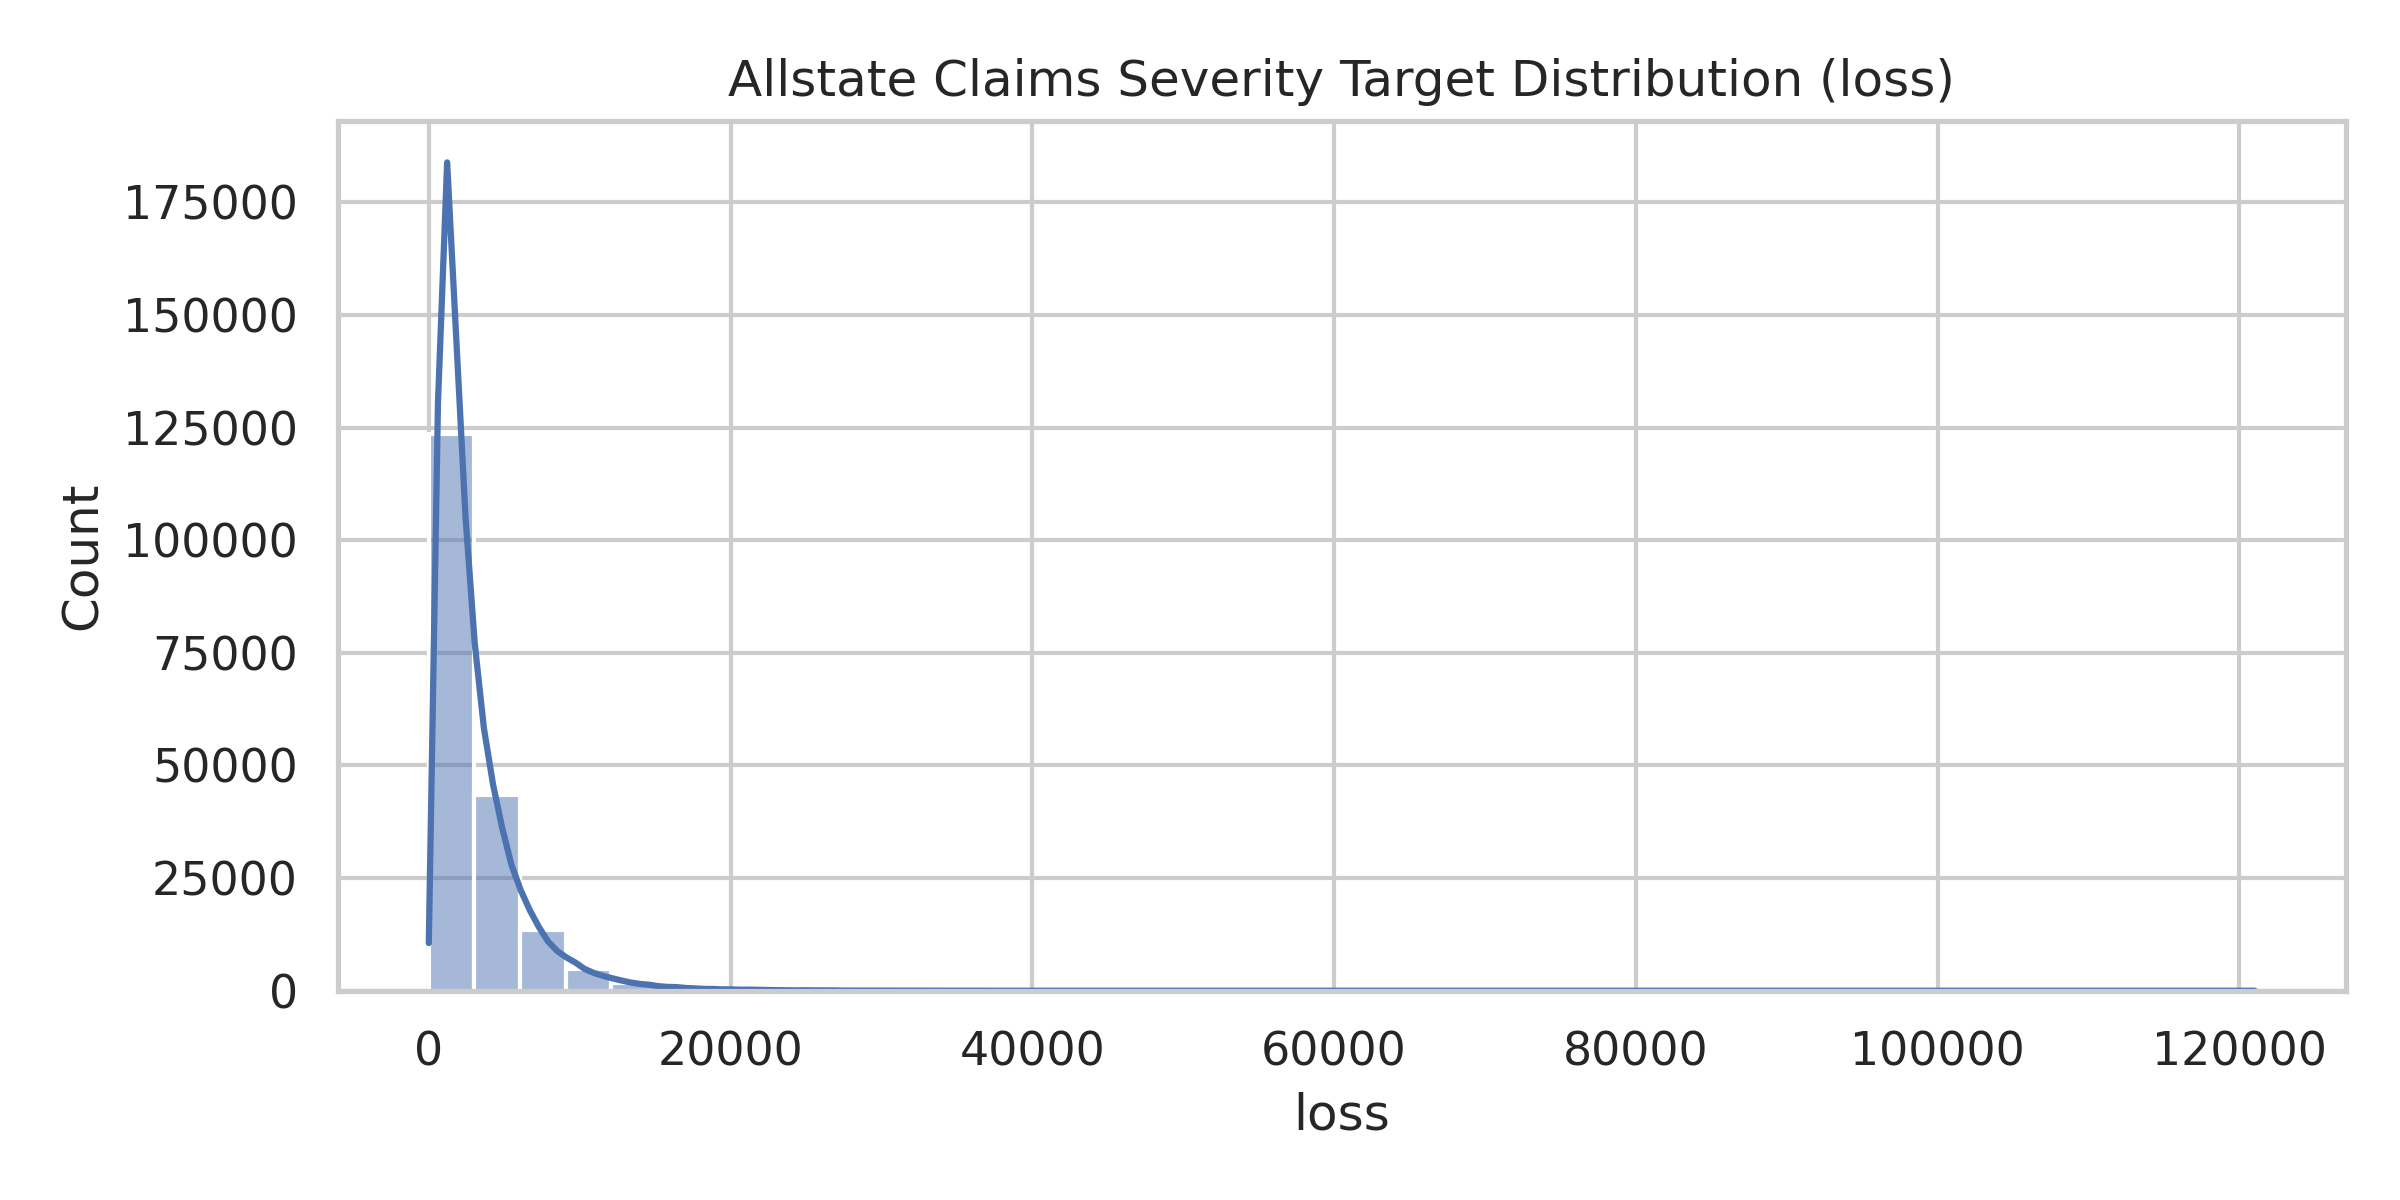
\includegraphics[width=0.65\textwidth]{../pre_study/figures/allstate_claims_target_distribution.png}\\[0.3em]
    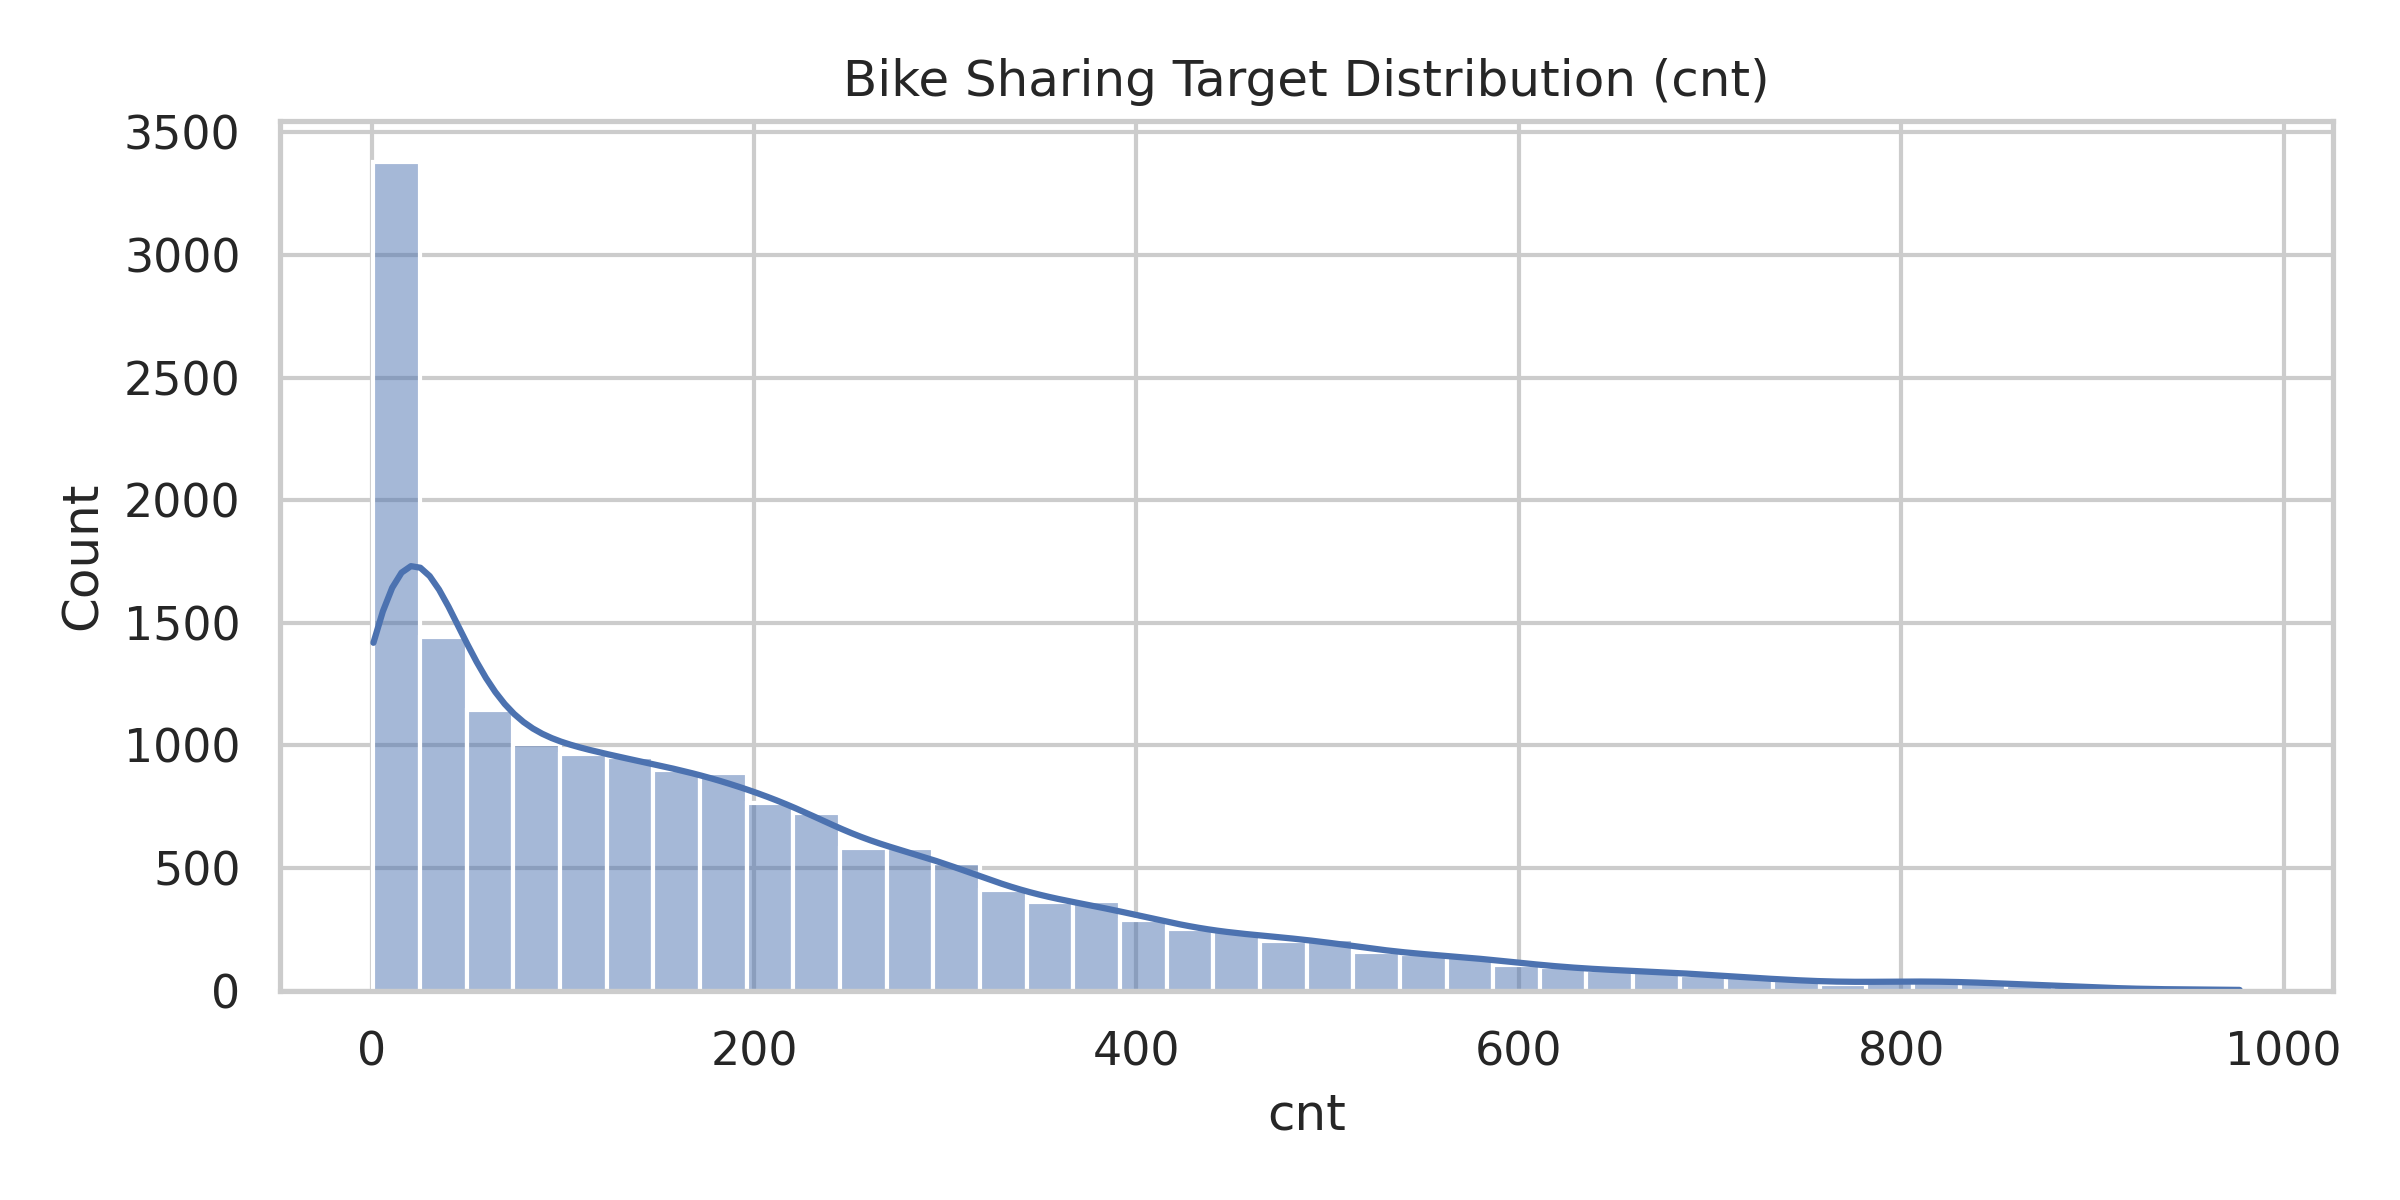
\includegraphics[width=0.65\textwidth]{../pre_study/figures/bike_sharing_target_distribution.png}\\[0.3em]
    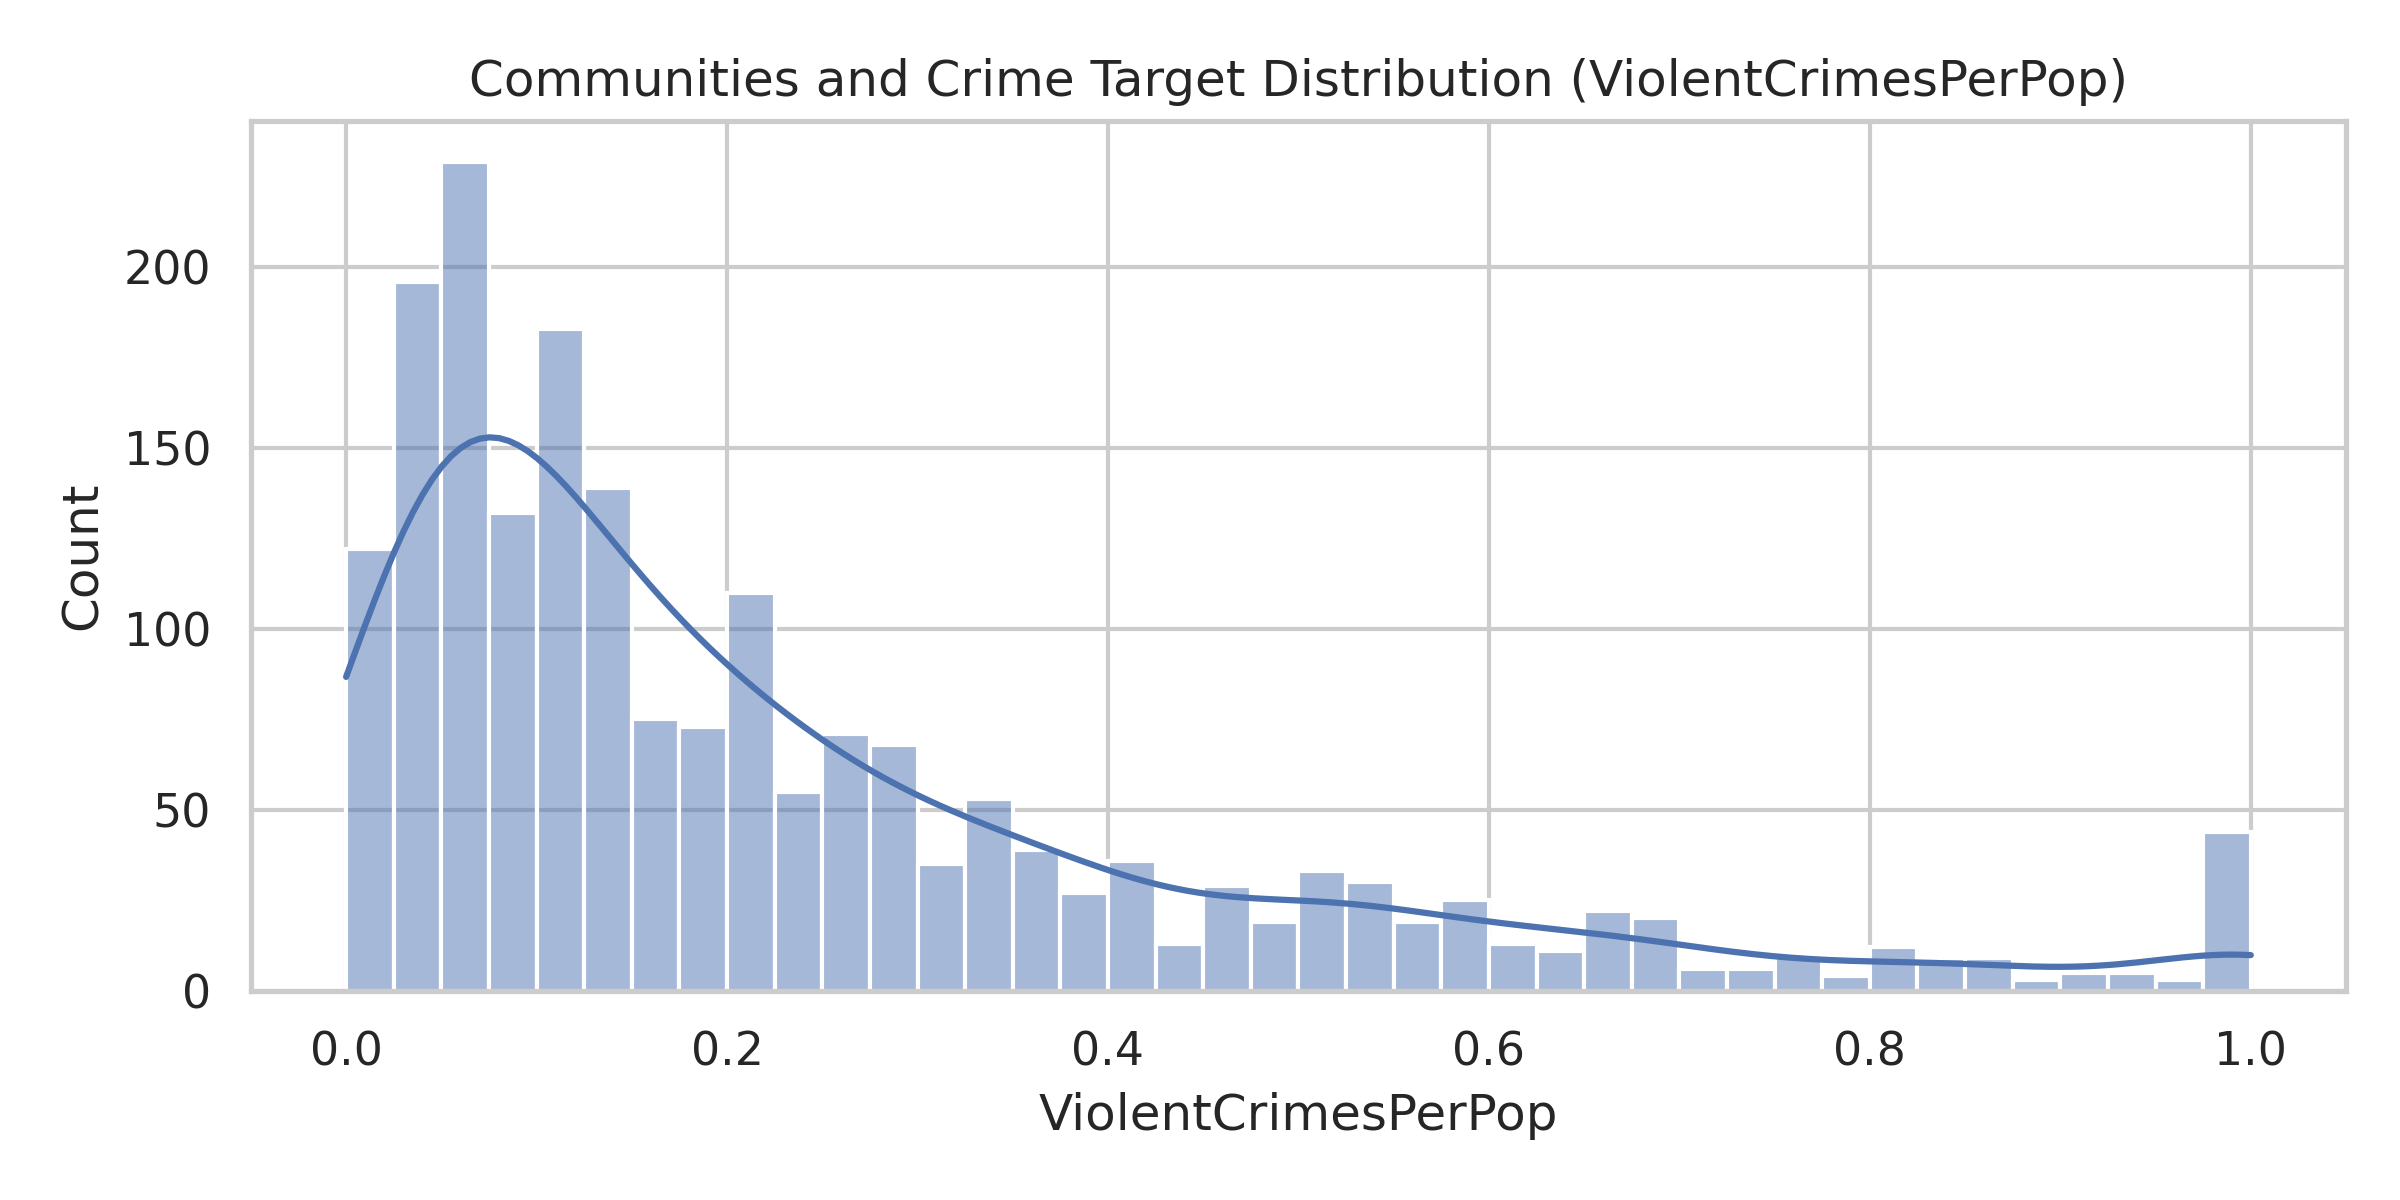
\includegraphics[width=0.65\textwidth]{../pre_study/figures/communities_crime_target_distribution.png}
    \caption{Target variable distributions for all four datasets.}
    \label{fig:target_dist}
\end{figure}

\begin{figure}[p]
    \centering
    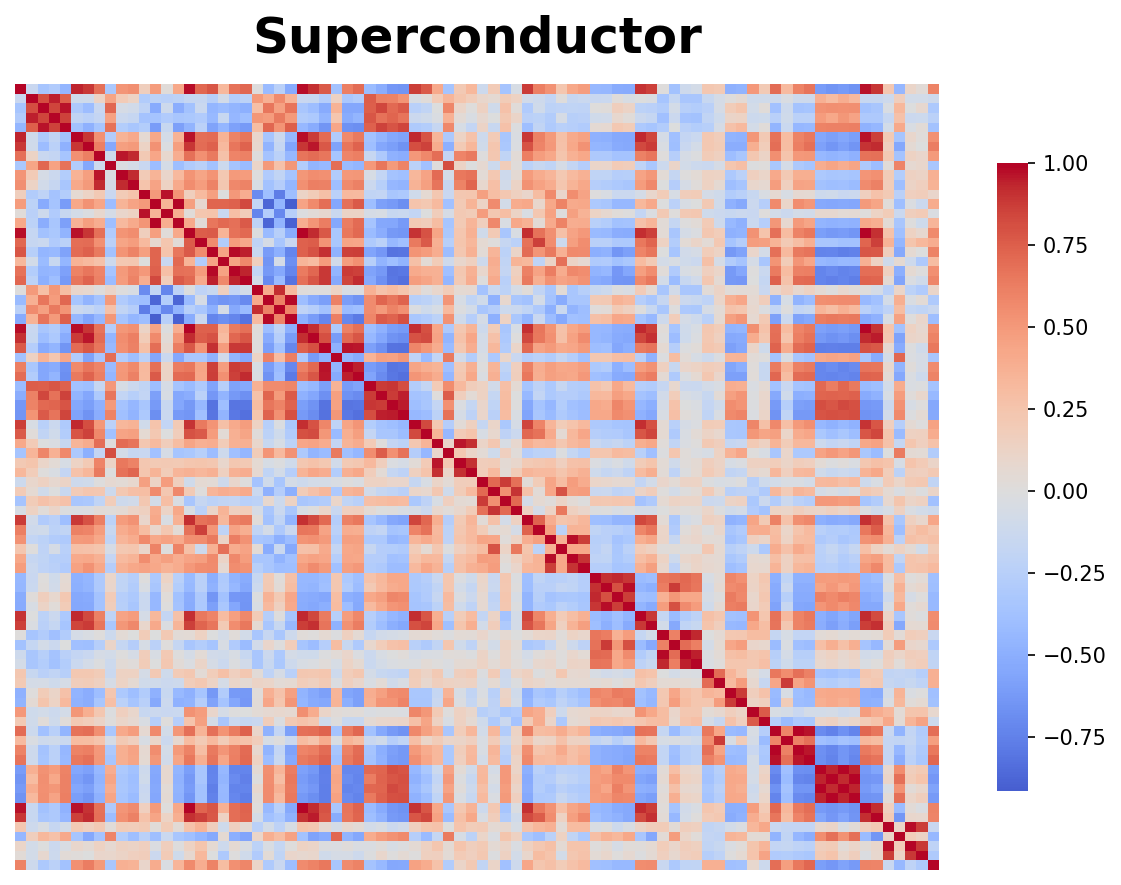
\includegraphics[width=0.48\textwidth]{../pre_study/figures/superconductor_correlation_heatmap.png}
    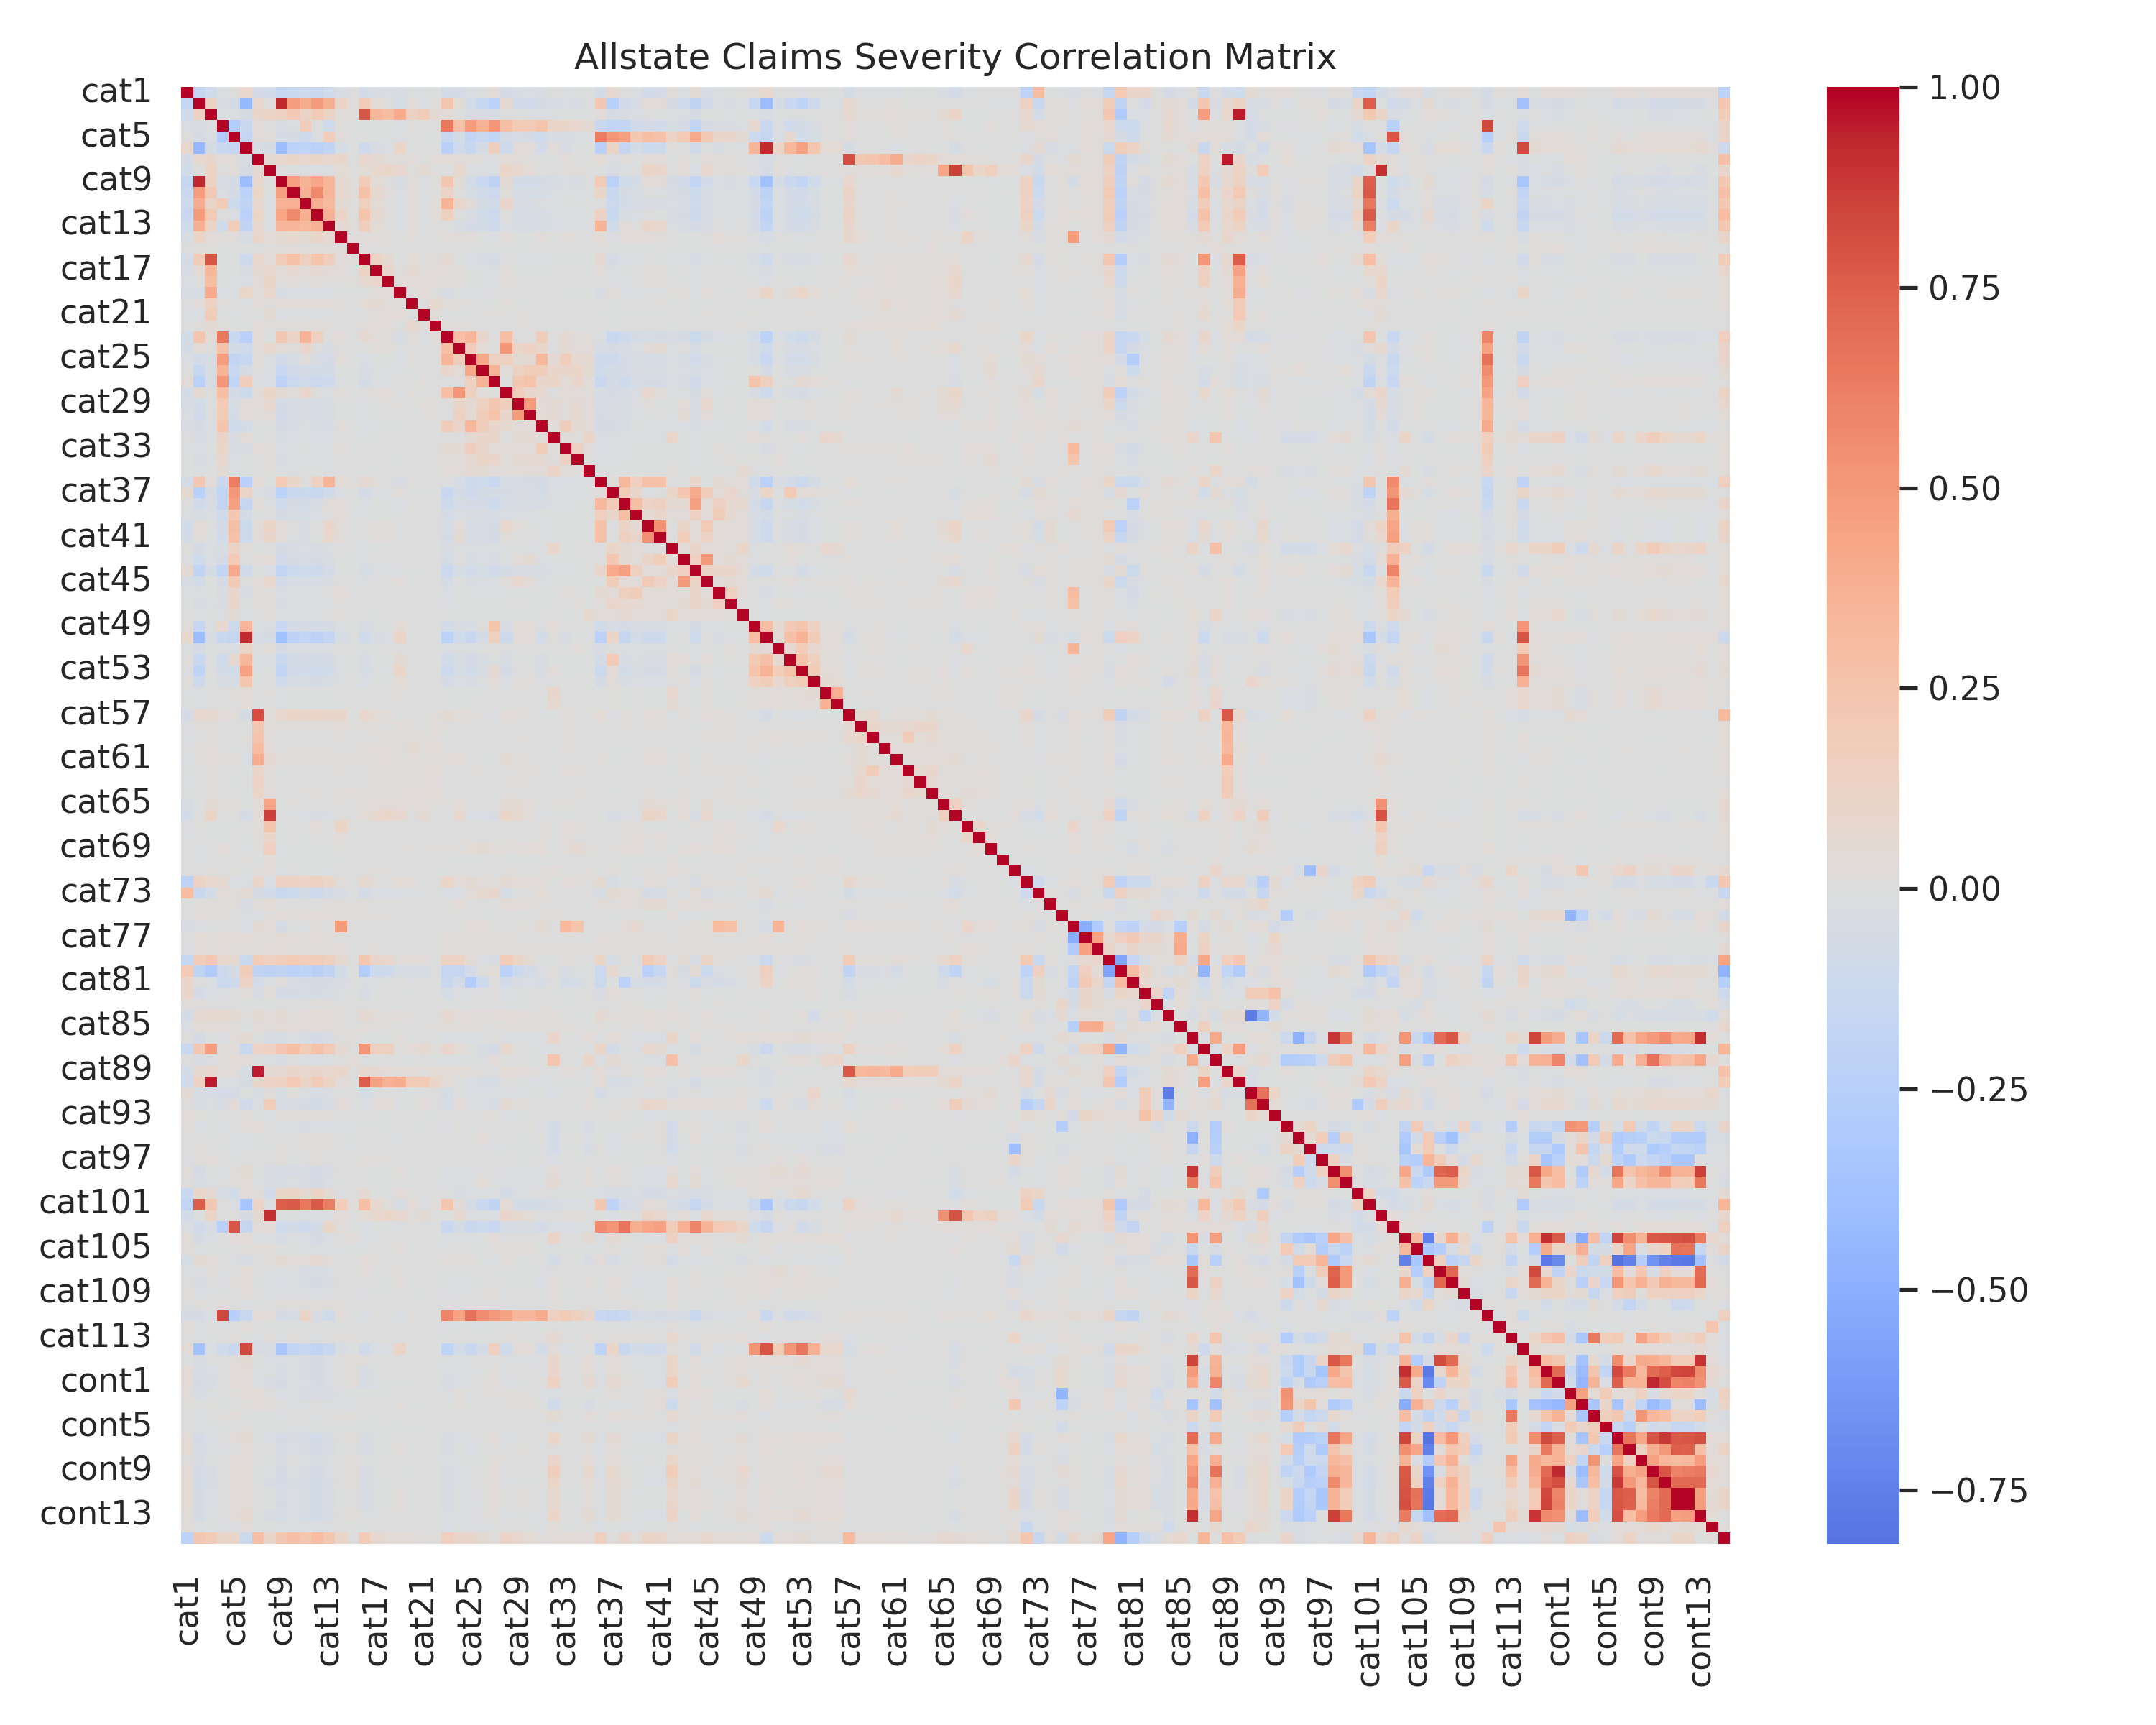
\includegraphics[width=0.48\textwidth]{../pre_study/figures/allstate_claims_correlation_heatmap.png}\\[0.5em]
    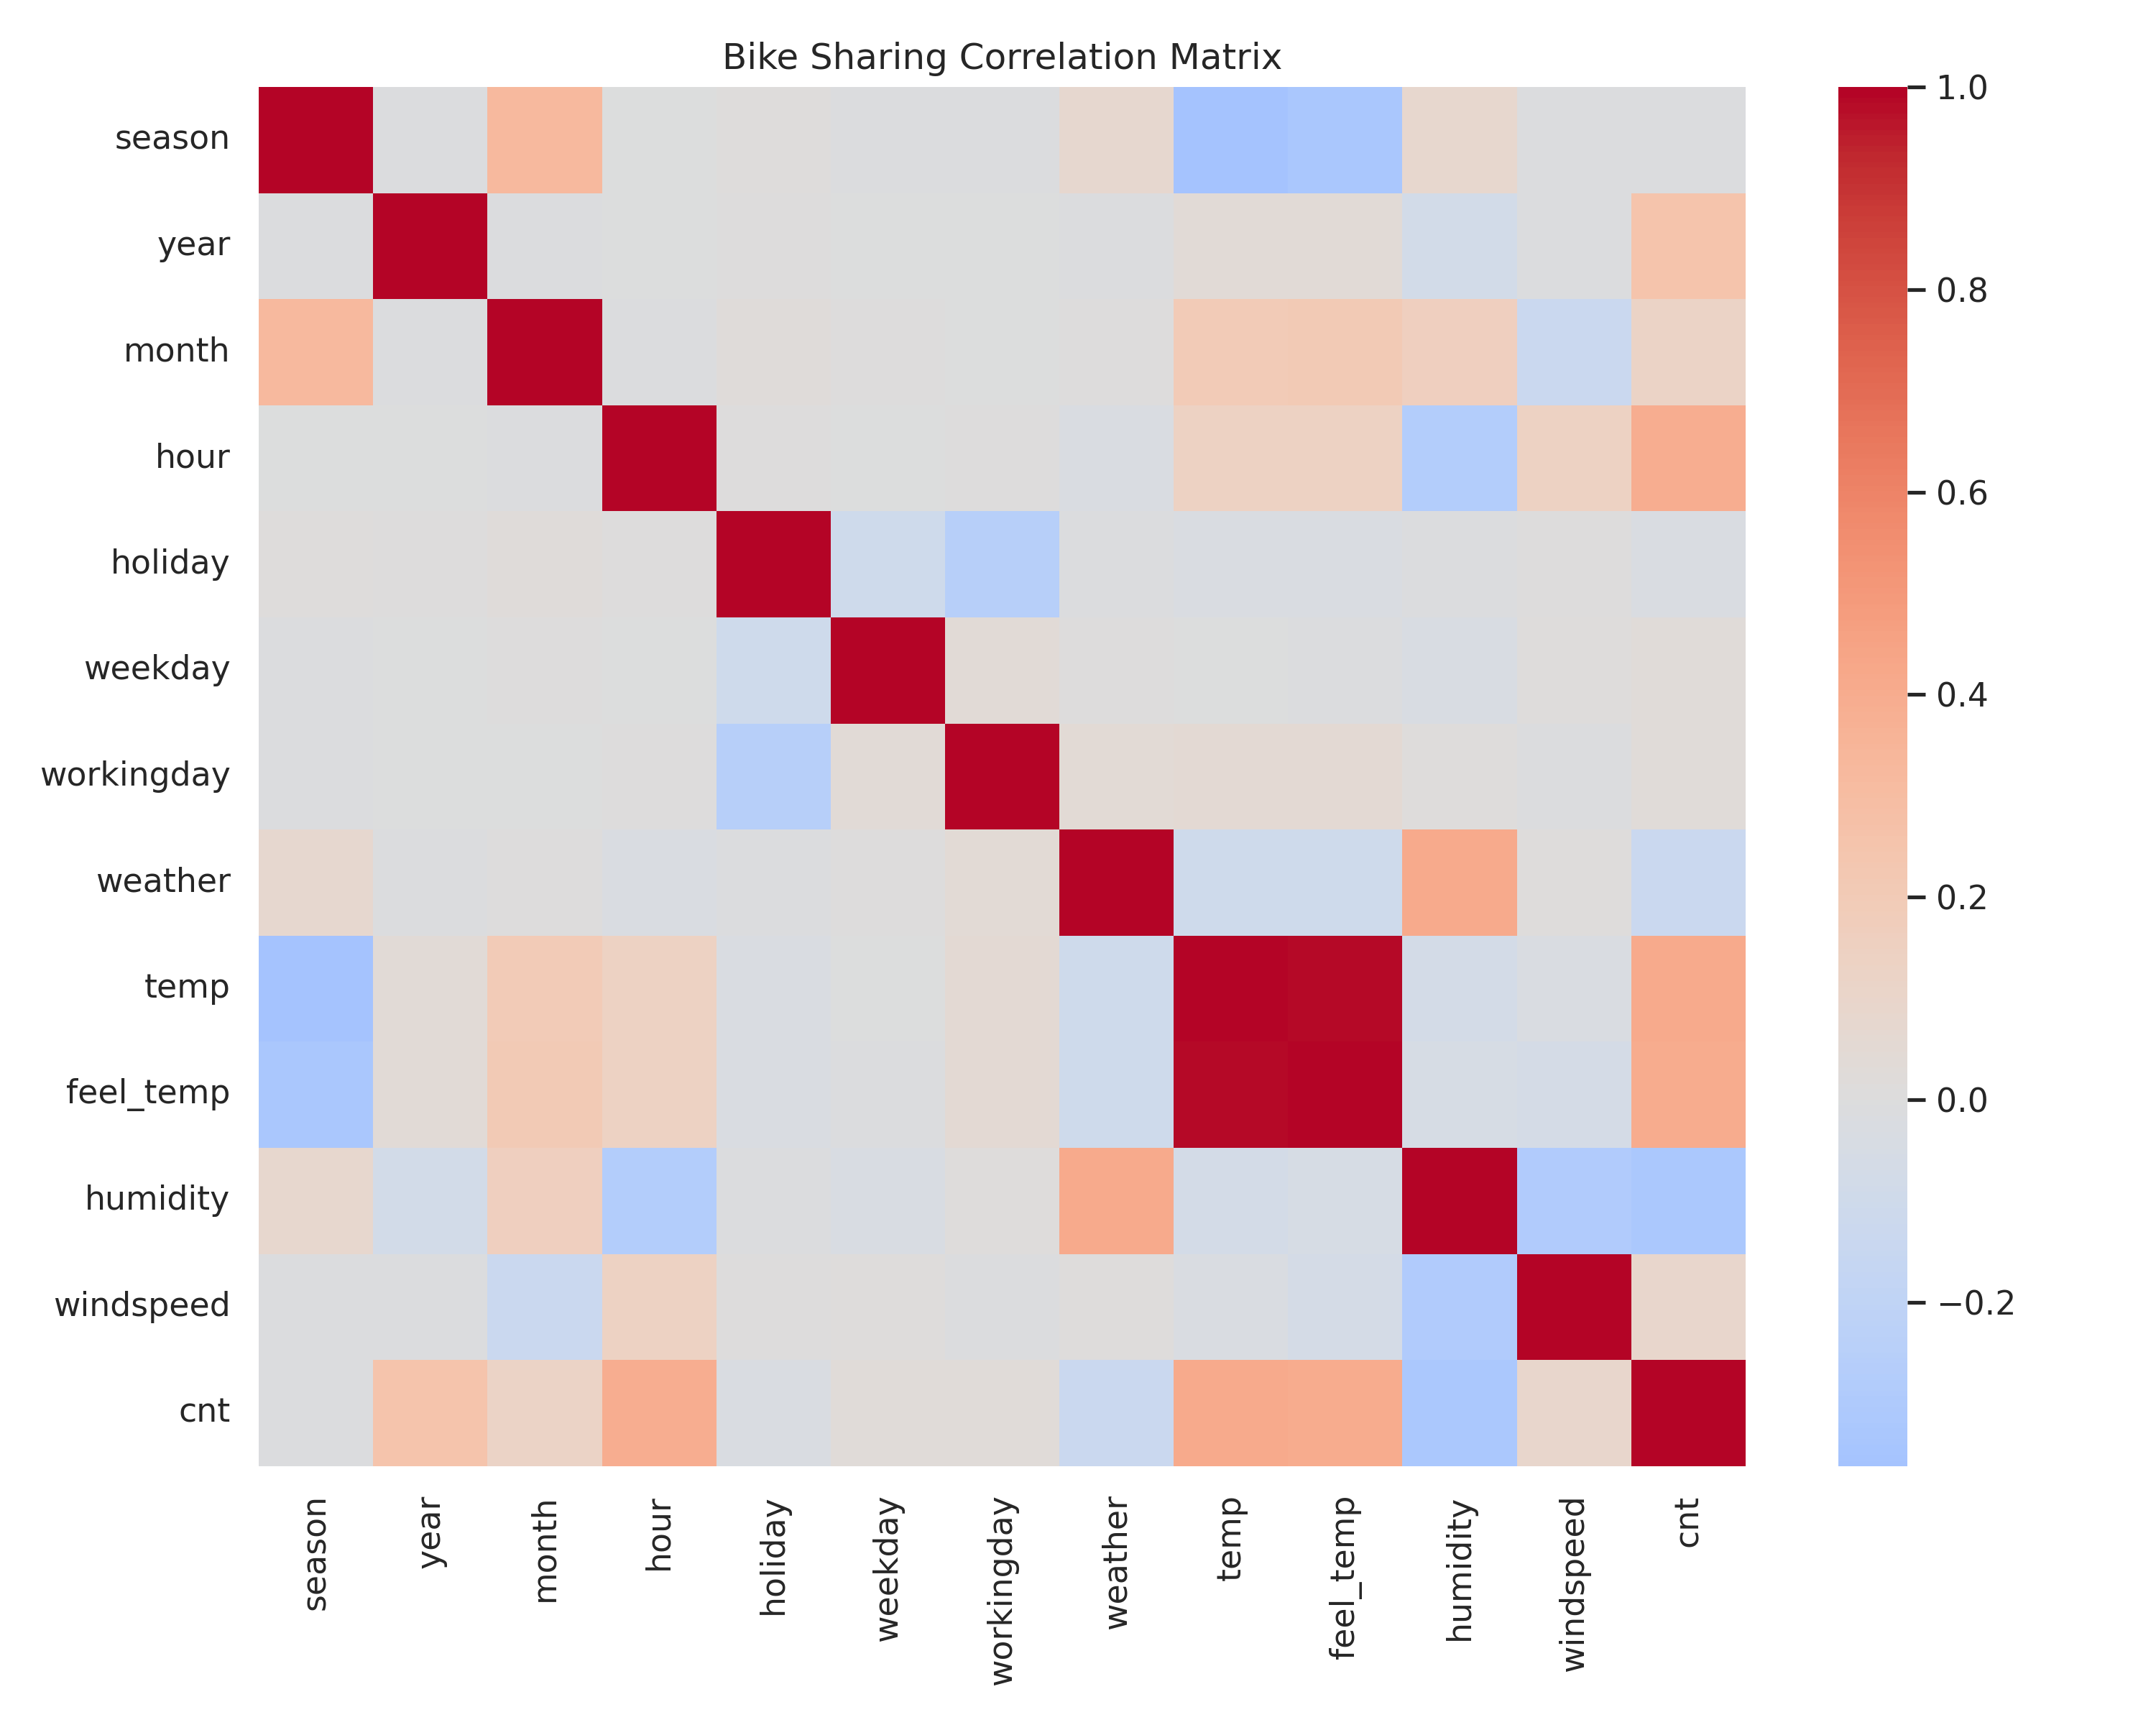
\includegraphics[width=0.48\textwidth]{../pre_study/figures/bike_sharing_correlation_heatmap.png}
    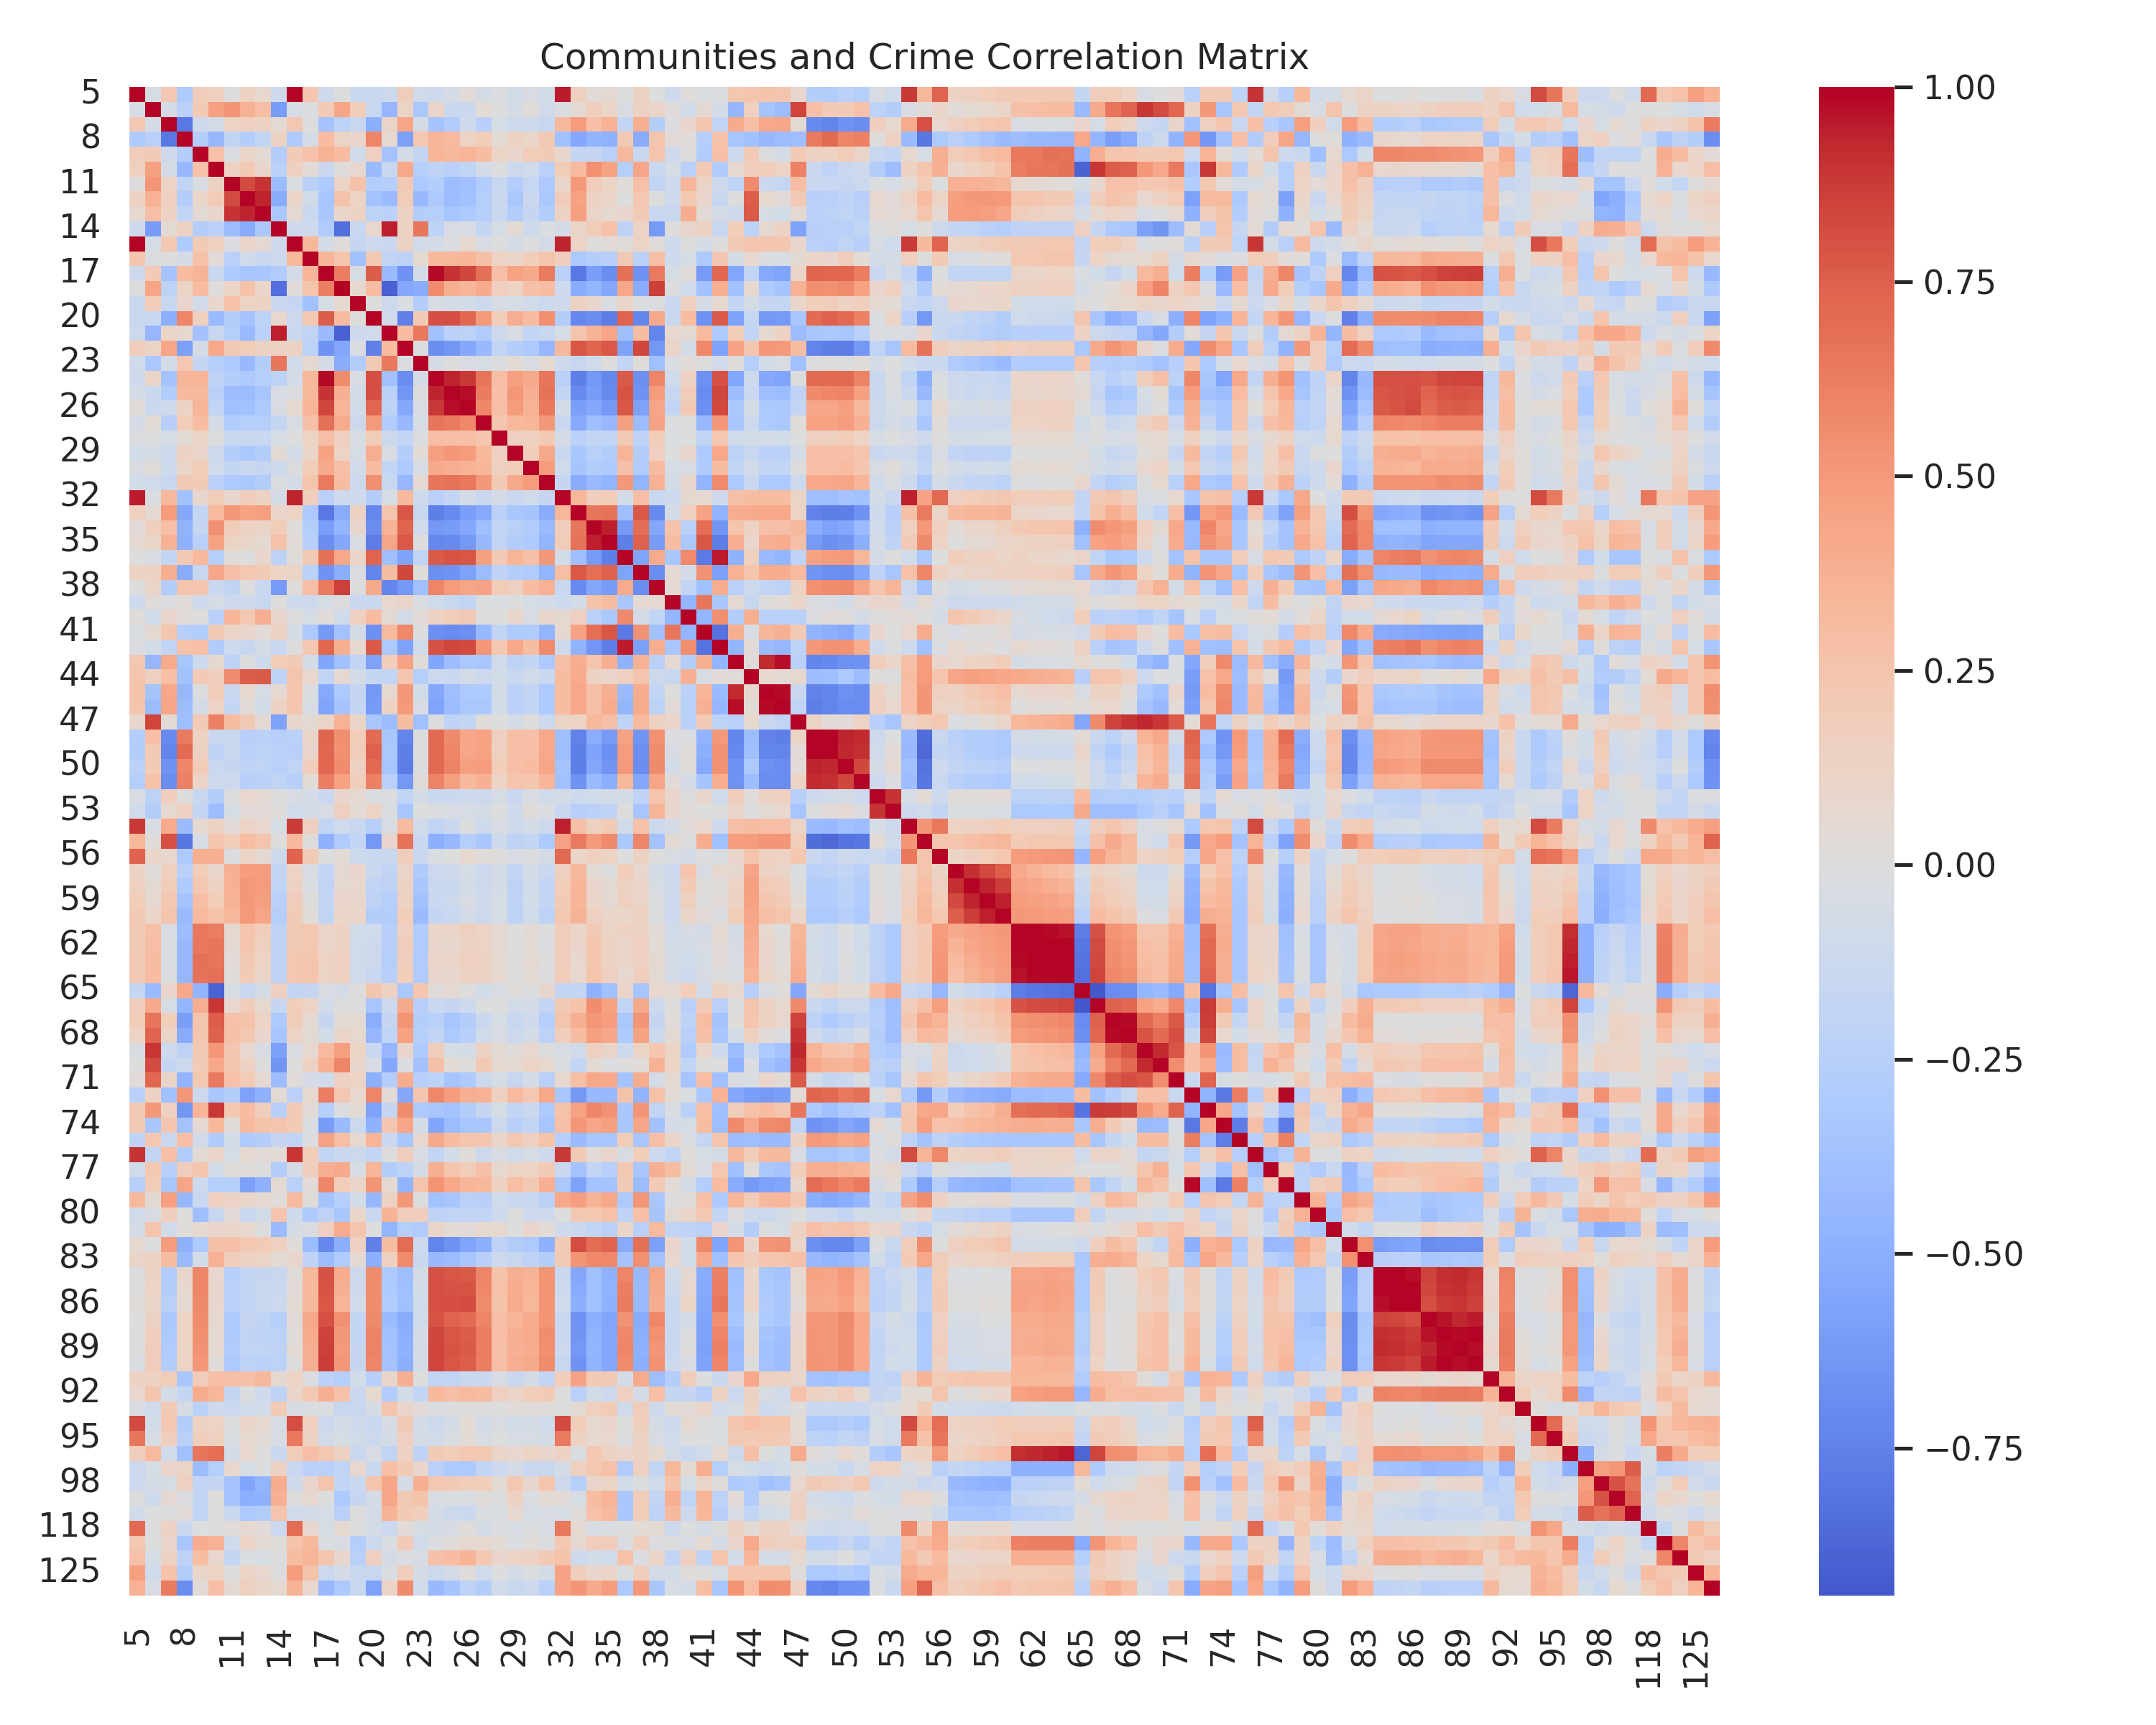
\includegraphics[width=0.48\textwidth]{../pre_study/figures/communities_crime_correlation_heatmap.png}
    \caption{Feature correlation heatmaps showing multicollinearity patterns across the four datasets.}
    \label{fig:correlation}
\end{figure}

\section{Chapter Summary}

This review has established the technical context for the experimental work. Regression on tabular data is best served by ensemble tree methods, though linear baselines remain useful references. Feature selection spans filter, wrapper, and embedded approaches, each with distinct trade-offs. SHAP provides theoretically principled feature attributions, and TreeExplainer makes exact computation tractable for tree models, though not without cost. The selected datasets span a meaningful range of sizes and structures, enabling evaluation of whether method performance generalizes. With this foundation in place, the next chapter formalizes the research hypotheses and experimental design.
